% Document settings
\documentclass[a4paper,11pt]{article}

% Packages
  % math formulas
\usepackage{amsmath,amsthm,amssymb}
  % graphics
\usepackage{graphicx}
\usepackage{wrapfig}
  % plots
\usepackage{pgfplots}
  % other
\usepackage[warn]{mathtext}
\usepackage{cmap}
\usepackage[T1,T2A]{fontenc}
\usepackage[utf8]{inputenc}
\usepackage[english,russian]{babel}

% Package settings
%% graphicx
\graphicspath{{Pictures/}}
\DeclareGraphicsExtensions{.pdf,.png,.jpg}
%% pgfplots
\pgfplotsset{width=10cm,compat=1.9}

% Title
\title{Отчет о выполнении работы №1.3.1\\Определение модуля Юнга.}
\author{Воейко Андрей Александрович, Б01-109}
\date{Долгопрудный, 2021}

% Document
\begin{document}
\maketitle
\newpage
\section{Аннотация.}
В работе экспериментально измеряется зависимость между напряжением и деформацией растяжения проволоки. По результатам измерений вычисляется модуль Юнга этой проволоки.
\section{Теоретические сведения.}
Растяжение проволоки соответствует случаю одноосного напряженного состояния, описываемого формулой~\ref{eq1}.
\begin{equation}    \label{eq1}
  \sigma = E \epsilon.
\end{equation}
В работе используется т. н. прибор Лермонтова, изображенный на рисунке~\ref{fig:img1}
\begin{wrapfigure}{r}{0.5\textwidth}
  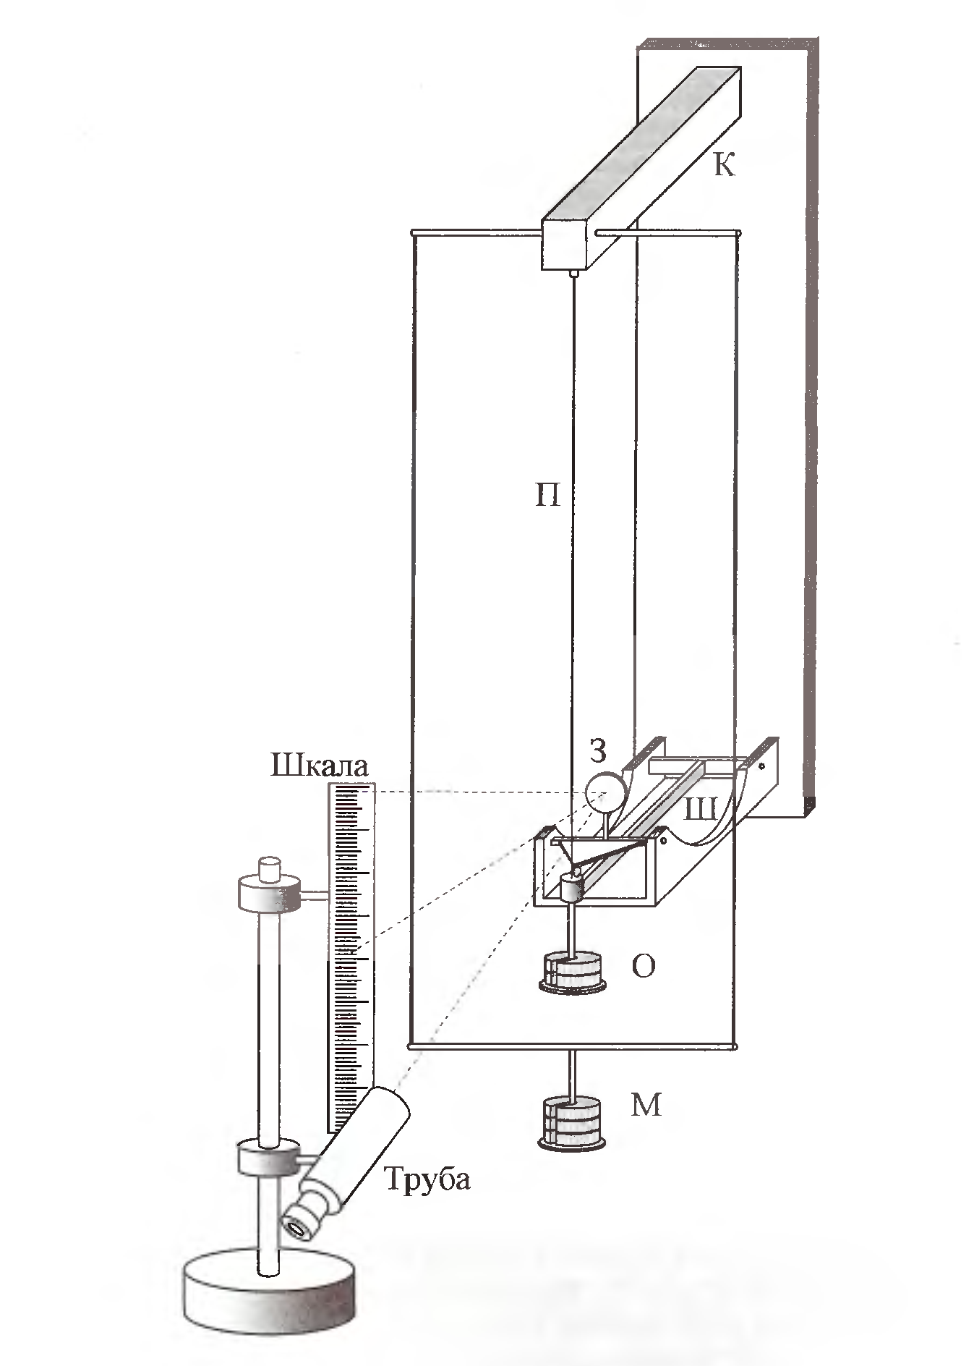
\includegraphics[scale = 0.3]{pic1.png}
  \caption{Прибор Лермонтова.}
  \label{fig:img1}
\end{wrapfigure}
Проволока $П$ одним концом закрепляется в кронштейне $К$, а другим прикреплена к подвешенному через шарнир кронштейну $Ш$. К этому же кронштейну снизу вешаются грузы на площадке $О$. Сами грузы хранятся на площадке $М$, висящей непосредственно на кронштейне $К$, для исключения влияния на результаты эксперимента деформации кронштейна $K$. Также к кронтштейну $Ш$ прикреплено зеркальце, по изменению угла наклона которго можно измерить деформацию проволоки. Угол наклона же вычисляется по изменению отражаемой части шкалы при наблюдении за ней из трубы. Вычисляется он по формуле~\ref{eq2}.
\begin{equation}    \label{eq2}
  \alpha = \frac{\Delta n}{h},
\end{equation}
где $\alpha$ -- это угол наклона зеркальца, $\Delta n$ -- изменение показания шкалы, $h$ -- расстояние от зеркальца до шкалы.
Формула для вычисления удленения проволоки:
\begin{equation}    \label{eq3}
  \Delta l = r \frac{\Delta n}{2h},
\end{equation}
где $\Delta l$ -- изменение длины проволоки, а $r$ -- длина рычажка зеркала.
\section{Оборудование и экспериментальная установка.}
В работе используются:
\begin{itemize}
  \item Прибор Лермонтова.
  \item Набор грузов.
  \item Шкала. Значение -- в сантиметрах, цена деления -- $1\ мм$.
  \item Длина рычажка -- $r = 20\ мм$.
  \item Расстояние от шкалы до зеркальца -- $h = 136,1 \pm 0,1\ см$.
  \item Длина проволоки -- $l = 173,2 \pm 0,1\ см$.
  \item Диаметр проволоки -- $d_{пр} = 0,51\ мм$.
\end{itemize}
\section{Результаты измерений и обработка данных.}
\subsection{Результаты измерений.}
Проведем измерения отражения шкалы в зеркальце, сначала добавляя, а затем убирая грузы с площадки $О$. Повторим измерения трижды. Результаты занесем в таблицу~\ref{table:tab1}.
% Табл. 1 {{{
\begin{table}[h!]
\centering
\begin{tabular}{ ||c|c|c|c|c|c|| }
  \hline
  \multicolumn{3}{||c|}{Серия измерений} & I & II & III \\
  \hline
  Номер & Масса & Изменение & & & \\
  верхнего & груза & веса груза & $n_{1}$, $мм$ & $n_{2}$, $мм$ & $n_{3}$, $мм$ \\
  груза $N_{гр}$ & $m_{гр}$, $г$ & $\Delta P_{гр}$, $Н$ & & & \\
  \hline
  $1$ & -- & -- & $8,3 \pm 0,1$ & $8,1 \pm 0,1$ & $8,3 \pm 0,1$ \\
  $2$ & $245,5$ & $+2,41$ & $10,1 \pm 0,1$ & $10,1 \pm 0,1$ & $10,1 \pm 0,1$ \\
  $3$ & $245,6$ & $+2,41$ & $11,9 \pm 0,1$ & $11,9 \pm 0,1$ & $12,0 \pm 0,1$ \\
  $4$ & $244,8$ & $+2,40$ & $13,6 \pm 0,1$ & $13,6 \pm 0,1$ & $13,7 \pm 0,1$ \\
  $5$ & $245,8$ & $+2,41$ & $15,1 \pm 0,1$ & $15,3 \pm 0,1$ & $15,2 \pm 0,1$ \\
  $6$ & $244,9$ & $+2,40$ & $16,8 \pm 0,1$ & $16,8 \pm 0,1$ & $16,9 \pm 0,1$ \\
  $7$ & $245,8$ & $+2,41$ & $18,3 \pm 0,1$ & $18,4 \pm 0,1$ & $18,5 \pm 0,1$ \\
  $8$ & $245,8$ & $+2,41$ & $20,0 \pm 0,1$ & $20,0 \pm 0,1$ & $20,2 \pm 0,1$ \\
  $9$ & $245,7$ & $+2,41$ & $21,6 \pm 0,1$ & $21,6 \pm 0,1$ & $21,7 \pm 0,1$ \\
  $10$ & $245,3$ & $+2,41$ & $23,2 \pm 0,1$ & $23,3 \pm 0,1$ & $23,2 \pm 0,1$ \\
  $9$ & $245,7$ & $-2,41$ & $21,6 \pm 0,1$ & $21,8 \pm 0,1$ & $21,6 \pm 0,1$ \\
  $8$ & $245,8$ & $-2,41$ & $20,1 \pm 0,1$ & $20,2 \pm 0,1$ & $20,2 \pm 0,1$ \\
  $7$ & $245,8$ & $-2,41$ & $18,6 \pm 0,1$ & $18,7 \pm 0,1$ & $18,6 \pm 0,1$ \\
  $6$ & $244,9$ & $-2,41$ & $17,1 \pm 0,1$ & $17,2 \pm 0,1$ & $17,1 \pm 0,1$ \\
  $5$ & $245,8$ & $-2,40$ & $15,3 \pm 0,1$ & $15,5 \pm 0,1$ & $15,5 \pm 0,1$ \\
  $4$ & $244,8$ & $-2,41$ & $13,7 \pm 0,1$ & $13,8 \pm 0,1$ & $13,7 \pm 0,1$ \\
  $3$ & $245,6$ & $-2,40$ & $12,0 \pm 0,1$ & $12,1 \pm 0,1$ & $12,0 \pm 0,1$ \\
  $2$ & $245,5$ & $-2,41$ & $10,2 \pm 0,1$ & $10,2 \pm 0,1$ & $10,3 \pm 0,1$ \\
  \hline
\end{tabular}
\caption{Результаты измерений.}
\label{table:tab1}
\end{table}
% }}}
\subsection{Обработка данных.}
\subsubsection{Подготовка данных для построения графиков.}
Составим таблицы~\ref{table:tab2}, \ref{table:tab3} и \ref{table:tab4} изменения длины проволоки в первой, второй и третьей сериях измерения соответственно.
% Табл. 2 {{{
\begin{table}[h!]
\centering
\begin{tabular}{ ||c|c|c|c|| }
  \hline
  Номер верхнего & Изменение веса & $\Delta n_{1}$, & $\Delta l_{1}$, \\
  груза $N_{гр}$ & груза $P_{гр}$, $Н$ & $мм$ & $мм$ \\
  \hline
  $1$ & $0,0$ & $0,0 \pm 0,2$ & $0,00 \pm 0,00015$ \\
  $2$ & $2,42$ & $1,8 \pm 0,2$ & $0,00132 \pm 0,00015$ \\
  $3$ & $4,82$ & $3,6 \pm 0,2$ & $0,00265 \pm 0,00015$ \\
  $4$ & $7,22$ & $5,3 \pm 0,2$ & $0,00389 \pm 0,00015$ \\
  $5$ & $9,63$ & $6,8 \pm 0,2$ & $0,00500 \pm 0,00015$ \\
  $6$ & $12,03$ & $8,5 \pm 0,2$ & $0,00625 \pm 0,00015$ \\
  $7$ & $14,44$ & $10,0 \pm 0,2$ & $0,00735 \pm 0,00015$ \\
  $8$ & $16,86$ & $11,7 \pm 0,2$ & $0,00860 \pm 0,00015$ \\
  $9$ & $19,27$ & $13,3 \pm 0,2$ & $0,00977 \pm 0,00015$ \\
  $10$ & $21,67$ & $14,9 \pm 0,2$ & $0,01095 \pm 0,00015$ \\
  $9$ & $19,27$ & $13,3 \pm 0,2$ & $0,00977 \pm 0,00015$ \\
  $8$ & $16,86$ & $11,8 \pm 0,2$ & $0,00867 \pm 0,00015$ \\
  $7$ & $14,44$ & $10,3 \pm 0,2$ & $0,00757 \pm 0,00015$ \\
  $6$ & $12,03$ & $8,8 \pm 0,2$ & $0,00647 \pm 0,00015$ \\
  $5$ & $9,63$ & $7,0 \pm 0,2$ & $0,00529 \pm 0,00015$ \\
  $4$ & $7,22$ & $5,4 \pm 0,2$ & $0,00397 \pm 0,00015$ \\
  $3$ & $4,82$ & $3,7 \pm 0,2$ & $0,00272 \pm 0,00015$ \\
  $2$ & $2,42$ & $1,9 \pm 0,2$ & $0,00140 \pm 0,00015$ \\
  \hline
\end{tabular}
\caption{Изменения длины проволоки в первой серии измерений.}
\label{table:tab2}
\end{table}
% }}}
% Табл. 3 {{{
\begin{table}[h!]
\centering
\begin{tabular}{ ||c|c|c|c|| }
  \hline
  Номер верхнего & Изменение веса & $\Delta n_{2}$, & $\Delta l_{2}$, \\
  груза $N_{гр}$ & груза $P_{гр}$, $Н$ & $мм$ & $мм$ \\
  \hline
  $1$ & $0,0$ & $0,0 \pm 0,2$ & $0,00 \pm 0,00015$ \\
  $2$ & $2,42$ & $2,0 \pm 0,2$ & $0,00147 \pm 0,00015$ \\
  $3$ & $4,82$ & $3,8 \pm 0,2$ & $0,00279 \pm 0,00015$ \\
  $4$ & $7,22$ & $5,5 \pm 0,2$ & $0,00404 \pm 0,00015$ \\
  $5$ & $9,63$ & $7,0 \pm 0,2$ & $0,00514 \pm 0,00015$ \\
  $6$ & $12,03$ & $8,7 \pm 0,2$ & $0,00639 \pm 0,00015$ \\
  $7$ & $14,44$ & $10,3 \pm 0,2$ & $0,00757 \pm 0,00015$ \\
  $8$ & $16,86$ & $11,9 \pm 0,2$ & $0,00874 \pm 0,00015$ \\
  $9$ & $19,27$ & $13,5 \pm 0,2$ & $0,00992 \pm 0,00015$ \\
  $10$ & $21,67$ & $15,2 \pm 0,2$ & $0,01168 \pm 0,00015$ \\
  $9$ & $19,27$ & $13,7 \pm 0,2$ & $0,01007 \pm 0,00015$ \\
  $8$ & $16,86$ & $12,1 \pm 0,2$ & $0,00889 \pm 0,00015$ \\
  $7$ & $14,44$ & $10,6 \pm 0,2$ & $0,00779 \pm 0,00015$ \\
  $6$ & $12,03$ & $9,1 \pm 0,2$ & $0,00669 \pm 0,00015$ \\
  $5$ & $9,63$ & $7,4 \pm 0,2$ & $0,00544 \pm 0,00015$ \\
  $4$ & $7,22$ & $5,7 \pm 0,2$ & $0,00419 \pm 0,00015$ \\
  $3$ & $4,82$ & $4,0 \pm 0,2$ & $0,00294 \pm 0,00015$ \\
  $2$ & $2,42$ & $2,1 \pm 0,2$ & $0,00154 \pm 0,00015$ \\
  \hline
\end{tabular}
\caption{Изменения длины проволоки во второй серии измерений.}
\label{table:tab3}
\end{table}
% }}}
% Табл. 4 {{{
\begin{table}[h!]
\centering
\begin{tabular}{ ||c|c|c|c|| }
  \hline
  Номер верхнего & Изменение веса & $\Delta n_{3}$, & $\Delta l_{3}$, \\
  груза $N_{гр}$ & груза $P_{гр}$, $Н$ & $мм$ & $мм$ \\
  \hline
  $1$ & $0,0$ & $0,0 \pm 0,2$ & $0,00 \pm 0,00015$ \\
  $2$ & $2,42$ & $2,0 \pm 0,2$ & $0,00147 \pm 0,00015$ \\
  $3$ & $4,82$ & $3,7 \pm 0,2$ & $0,00272 \pm 0,00015$ \\
  $4$ & $7,22$ & $5,4 \pm 0,2$ & $0,00397 \pm 0,00015$ \\
  $5$ & $9,63$ & $6,9 \pm 0,2$ & $0,00507 \pm 0,00015$ \\
  $6$ & $12,03$ & $8,6 \pm 0,2$ & $0,00632 \pm 0,00015$ \\
  $7$ & $14,44$ & $10,2 \pm 0,2$ & $0,00749 \pm 0,00015$ \\
  $8$ & $16,86$ & $11,9 \pm 0,2$ & $0,00874 \pm 0,00015$ \\
  $9$ & $19,27$ & $13,4 \pm 0,2$ & $0,00985 \pm 0,00015$ \\
  $10$ & $21,67$ & $14,9 \pm 0,2$ & $0,01095 \pm 0,00015$ \\
  $9$ & $19,27$ & $13,3 \pm 0,2$ & $0,00977 \pm 0,00015$ \\
  $8$ & $16,86$ & $11,9 \pm 0,2$ & $0,00874 \pm 0,00015$ \\
  $7$ & $14,44$ & $10,3 \pm 0,2$ & $0,00757 \pm 0,00015$ \\
  $6$ & $12,03$ & $8,8 \pm 0,2$ & $0,00647 \pm 0,00015$ \\
  $5$ & $9,63$ & $7,2 \pm 0,2$ & $0,00529 \pm 0,00015$ \\
  $4$ & $7,22$ & $5,4 \pm 0,2$ & $0,00397 \pm 0,00015$ \\
  $3$ & $4,82$ & $3,7 \pm 0,2$ & $0,00272 \pm 0,00015$ \\
  $2$ & $2,42$ & $2,0 \pm 0,2$ & $0,00147 \pm 0,00015$ \\
  \hline
\end{tabular}
\caption{Изменения длины проволоки в третьей серии измерений.}
\label{table:tab4}
\end{table}
% }}}
\subsubsection{Графики зависимости изменения длины от веса грузов.}
На основании данных из предыдущего пункта построим графики зависимости изменения длины от веса грузов для каждой серии измерений на рисунках~2, 3 и 4. Аппроксимируем данные всех трех серий измерений к прямой $\Delta l = \beta P_{гр}$, где $\beta = \frac{1}{k} = \frac{l}{ES}$.
$$\beta = \frac{\left<xy\right> - \left<x\right>\left<y\right>}{\left<x^{2}\right> - \left<x\right>^{2}} = \frac{0,0818 - 0,0621}{157,5-117,4} = \frac{0,0197}{40,1} = $$
$$= 4,91 \cdot 10^{-4}\ \frac{мм}{Н} = 4,91 \cdot 10^{-7}\ \frac{м}{Н}$$
$$E = \frac{l}{\frac{\pi}{4}d^{2}\beta} = 1,72 \cdot 10^{11} \pm 0.3 \cdot 10^{11}\ \frac{Н}{м^{2}}$$
\begin{center}
\begin{tikzpicture}
\begin{axis}[
	xlabel = {$P_{гр}$},
	ylabel = {$\Delta l_{1}$},
    grid = major,
	minor tick num = 6
]
\addplot[
    blue,
    mark size = 2 pt,
    only marks,
]
table {
	x    y
  0.0   0.00
  2.42  0.00132
  4.82  0.00265
  7.22  0.00389
  9.63  0.00500
  12.03 0.00625
  14.44 0.00735
  16.86 0.00860
  19.27 0.00977
  21.67 0.01095
  19.27 0.00977
  16.86 0.00867
  14.44 0.00757
  12.03 0.00647
  9.63  0.00529
  7.22  0.00397
  4.82  0.00272
  2.42  0.00140
};
\end{axis}
\end{tikzpicture}\newline
Рис. 2: График зависимости изменения длины от веса грузов в первой серии измерений.
\end{center}
\begin{center}
\begin{tikzpicture}
\begin{axis}[
	xlabel = {$P_{гр}$},
	ylabel = {$\Delta l_{2}$},
    grid = major,
	minor tick num = 6
]
\addplot[
    green,
    mark size = 2 pt,
    only marks,
]
table {
	x    y
  0.0   0.00
  2.42  0.00147
  4.82  0.00279
  7.22  0.00404
  9.63  0.00514
  12.03 0.00639
  14.44 0.00757
  16.86 0.00874
  19.27 0.00992
  21.67 0.01168
  19.27 0.01007
  16.86 0.00889
  14.44 0.00779
  12.03 0.00669
  9.63  0.00544
  7.22  0.00419
  4.82  0.00294
  2.42  0.00154
};
\end{axis}
\end{tikzpicture}\newline
Рис. 3: График зависимости изменения длины от веса грузов во второй серии измерений.
\end{center}
\begin{center}
\begin{tikzpicture}
\begin{axis}[
	xlabel = {$P_{гр}$},
	ylabel = {$\Delta l_{3}$},
    grid = major,
	minor tick num = 6
]
\addplot[
    red,
    mark size = 2 pt,
    only marks,
]
table {
	x     y
  0.0   0.00
  2.42  0.00147
  4.82  0.00272
  7.22  0.00397
  9.63  0.00507
  12.03 0.00632
  14.44 0.00749
  16.86 0.00874
  19.27 0.00985
  21.67 0.01095
  19.27 0.00977
  16.86 0.00874
  14.44 0.00757
  12.03 0.00647
  9.63  0.00529
  7.22  0.00397
  4.82  0.00272
  2.42  0.00147
};
\end{axis}
\end{tikzpicture}\newline
Рис. 4: График зависимости изменения длины от веса грузов в третьей серии измерений.
\end{center}
\section{Выводы.}
В ходе работы был найден модуль Юнга материала проволоки, составивший $1,72 \cdot 10^{11} \pm 0,03 \cdot 10 ^{11} \frac{Н}{м^{2}}$. Он близок к модулю Юнга железа ($1,9 \cdot 10^{11}$ -- $2 \cdot 10^{11}\ \frac{Н}{м}$), но несколько ниже его. Скорее всего сказалось постепенное растяжение проволоки со временем, приведшее к ее истончению.
\end{document}
